\section{Calibration}
SOLTI Calibration is a commonly used calibration method in network analyzers. SOL stands for Short-Open-Load, the standards that are commonly used for a single port calibration. In order to calibrate the s-parameters between different ports, also Through-Isolation (TI) can be used to calibrate S21 and S12.




\subsection{SOL Calibration}
\label{sec:solcal}

\begin{figure}[H]
	\centering
	\input{figures/OnePortModel.tex}
	\caption{One port model}
	\label{fig:oneportmodel}
\end{figure}


The measured S-parameter data can be de-embedded to the actual DUT with the lengths of the cables and the error coefficients of the network analyzer taken out of the data as if the DUT was measured directly.
	\begin{equation}
	\label{eqn:solcal}
	S11=\frac{S11_{M}-e_{00}}{(S11_{M}e_{11})-\Delta_{e}}
	\end{equation}
	\begin{itemize}
		\item $e_{00}$ is the Directivity
		\item $e_{11}$ is the port match
		\item $\Delta_{e} = e_{00}e_{11}-(e_{10}e_{01})$, of which $(e_{10}e_{01})$ is the tracking.
		\item $S11$ is the one port S-parameter that you want to display (De-embedded)
		\item 	$S11_M$ is the measured S-parameter including the cable and the errors of the port
	\end{itemize}

	The 3 error coefficients can be obtained from 3 independent measurements of known standards. The commonly used standards are Short, Open and Load, but any known standard can be used instead. (see section \ref{sec:obtainingerrorcoefsSOL})
\newpage
\subsubsection{Obtaining error coefficients for SOL calibration}
\label{sec:obtainingerrorcoefsSOL}

Equation \ref{eqn:solcal} contains 3 error coefficients $e_{00}$, $e_{11}$ and $\Delta_{e}$. From \cite{agilent_calibration} the equations \ref{eqn:obtaining1}, \ref{eqn:obtaining2} and \ref{eqn:obtaining3} are obtained. We see 3 times the same equations, but with different measurements. $\Gamma_1$, $\Gamma_2$ and $\Gamma_3$ are the known independent calibration standards, in this case Short, Open and Load. The standards don't have to be perfect though, a short can for instance have some series inductance or loss (see \ref{sec:calstds}). $\Gamma_{M1}$, $\Gamma_{M2}$ and $\Gamma_{M3}$ are the measured traces, this data is obtained by connecting the well-defined calibration standard to the network analyzer, through the cable that is also used in the measurement and measure the reflection (S11). Equations \ref{eqn:obtaining1}, \ref{eqn:obtaining2} and \ref{eqn:obtaining3} still contain our 3 unknown error coefficients $e_{00}$, $e_{11}$ and $\Delta_{e}$ that we need to solve equation \ref{eqn:solcal}.

	
	\small
	\begin{equation}
	\label{eqn:obtaining1}
	\Gamma_{M{1}} = e_{00}+\Gamma_{1}\Gamma_{M{1}}e{11}-\Gamma_{1}\Delta_{e}
	\end{equation}

	\begin{equation}
	\label{eqn:obtaining2}
	\Gamma_{M{2}} = e_{00}+\Gamma_{2}\Gamma_{M{2}}e{11}-\Gamma_{2}\Delta_{e}
	\end{equation}

	\begin{equation}
	\label{eqn:obtaining3}
	\Gamma_{M{3}} = e_{00}+\Gamma_{3}\Gamma_{M{3}}e{11}-\Gamma_{3}\Delta_{e}
	\end{equation}
	\normalsize

In order to solve $e_{00}$, $e_{11}$ and $\Delta_{e}$ we need to substitute equations  \ref{eqn:obtaining1}, \ref{eqn:obtaining2} and \ref{eqn:obtaining3} into one equation and extract the 3 error coefficients. The result is 3 lengthy equations, but with modern computers they can easily be computed for all the data points in our measurement.

	\small
	\begin{equation}
	\label{eqn:e00}
		e_{00} = -\frac{{\left(\Gamma_{2} \Gamma_{M_{3}} - \Gamma_{3} \Gamma_{M_{3}}\right)} \Gamma_{1} \Gamma_{M_{2}} - {\left(\Gamma_{2} \Gamma_{3} \Gamma_{M_{2}} - \Gamma_{2} \Gamma_{3} \Gamma_{M_{3}} - {\left(\Gamma_{3} \Gamma_{M_{2}} - \Gamma_{2} \Gamma_{M_{3}}\right)} \Gamma_{1}\right)} \Gamma_{M_{1}}}{\Gamma_{1} {\left(\Gamma_{2} - \Gamma_{3}\right)} \Gamma_{M_{1}} + \Gamma_{2} \Gamma_{3} \Gamma_{M_{2}} - \Gamma_{2} \Gamma_{3} \Gamma_{M_{3}} - {\left(\Gamma_{2} \Gamma_{M_{2}} - \Gamma_{3} \Gamma_{M_{3}}\right)} \Gamma_{1}}		
	\end{equation}
	\begin{equation}
	\label{eqn:e11}
	e_{11} = \frac{{\left(\Gamma_{2} - \Gamma_{3}\right)} \Gamma_{M_{1}} - \Gamma_{1} {\left(\Gamma_{M_{2}} - \Gamma_{M_{3}}\right)} + \Gamma_{3} \Gamma_{M_{2}} - \Gamma_{2} \Gamma_{M_{3}}}{\Gamma_{1} {\left(\Gamma_{2} - \Gamma_{3}\right)} \Gamma_{M_{1}} + \Gamma_{2} \Gamma_{3} \Gamma_{M_{2}} - \Gamma_{2} \Gamma_{3} \Gamma_{M_{3}} - {\left(\Gamma_{2} \Gamma_{M_{2}} - \Gamma_{3} \Gamma_{M_{3}}\right)} \Gamma_{1}}
	\end{equation}
	\begin{equation}
	\label{eqn:deltae}
	 \Delta_{e} = -\frac{{\left(\Gamma_{1} {\left(\Gamma_{M_{2}} - \Gamma_{M_{3}}\right)} - \Gamma_{2} \Gamma_{M_{2}} + \Gamma_{3} \Gamma_{M_{3}}\right)} \Gamma_{M_{1}} + {\left(\Gamma_{2} \Gamma_{M_{3}} - \Gamma_{3} \Gamma_{M_{3}}\right)} \Gamma_{M_{2}}}{\Gamma_{1} {\left(\Gamma_{2} - \Gamma_{3}\right)} \Gamma_{M_{1}} + \Gamma_{2} \Gamma_{3} \Gamma_{M_{2}} - \Gamma_{2} \Gamma_{3} \Gamma_{M_{3}} - {\left(\Gamma_{2} \Gamma_{M_{2}} - \Gamma_{3} \Gamma_{M_{3}}\right)} \Gamma_{1}}
	\end{equation}
	\normalsize
	
\newpage
\subsection{Full two port calibration}
\label{sec:soltical}
\begin{figure}[H]
	\centering
	% Graphic for TeX using PGF
% Title: /home/franss/DeEmbed/deembed/doc/figures/TwoPortModel.dia
% Creator: Dia v0.97.3
% CreationDate: Tue Jan 31 15:33:28 2017
% For: franss
% \usepackage{tikz}
% The following commands are not supported in PSTricks at present
% We define them conditionally, so when they are implemented,
% this pgf file will use them.
\ifx\du\undefined
  \newlength{\du}
\fi
\setlength{\du}{15\unitlength}
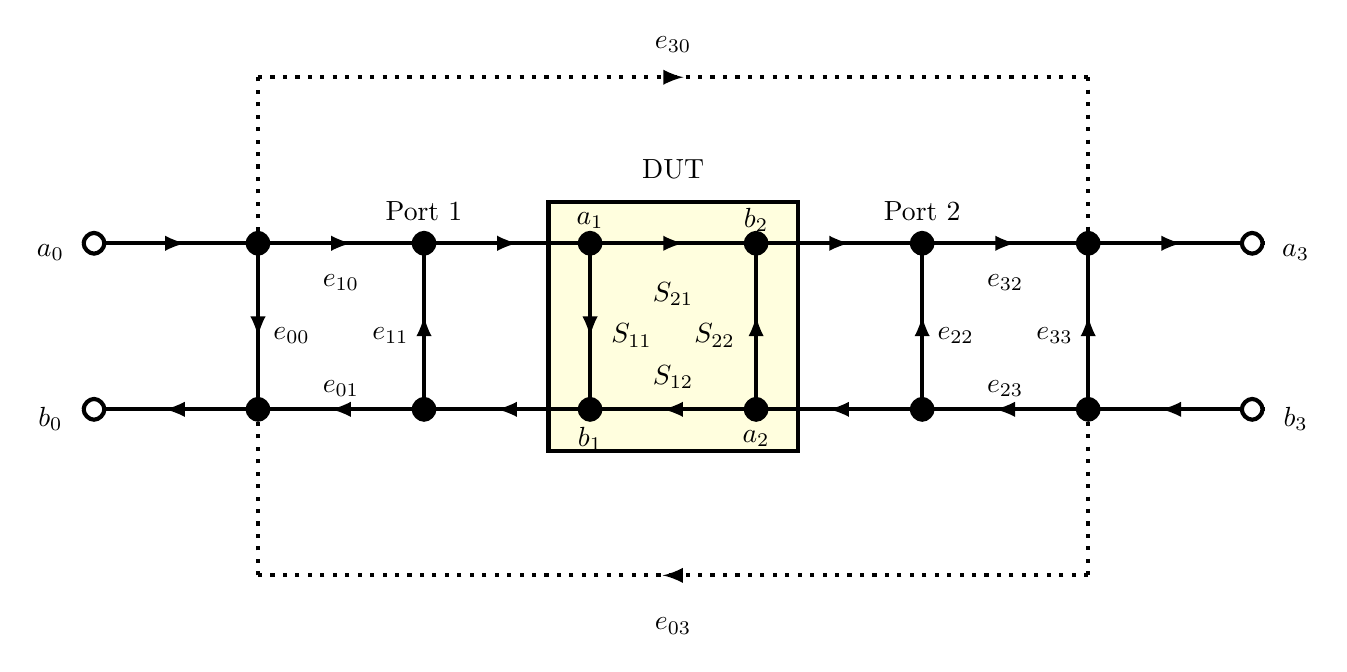
\begin{tikzpicture}
\pgftransformxscale{1.000000}
\pgftransformyscale{-1.000000}
\definecolor{dialinecolor}{rgb}{0.000000, 0.000000, 0.000000}
\pgfsetstrokecolor{dialinecolor}
\definecolor{dialinecolor}{rgb}{1.000000, 1.000000, 1.000000}
\pgfsetfillcolor{dialinecolor}
\definecolor{dialinecolor}{rgb}{1.000000, 0.996078, 0.870588}
\pgfsetfillcolor{dialinecolor}
\fill (34.000000\du,59.000000\du)--(34.000000\du,65.000000\du)--(40.000000\du,65.000000\du)--(40.000000\du,59.000000\du)--cycle;
\pgfsetlinewidth{0.100000\du}
\pgfsetdash{}{0pt}
\pgfsetdash{}{0pt}
\pgfsetmiterjoin
\definecolor{dialinecolor}{rgb}{0.000000, 0.000000, 0.000000}
\pgfsetstrokecolor{dialinecolor}
\draw (34.000000\du,59.000000\du)--(34.000000\du,65.000000\du)--(40.000000\du,65.000000\du)--(40.000000\du,59.000000\du)--cycle;
% setfont left to latex
\definecolor{dialinecolor}{rgb}{0.000000, 0.000000, 0.000000}
\pgfsetstrokecolor{dialinecolor}
\node at (37.000000\du,62.195000\du){};
\pgfsetlinewidth{0.100000\du}
\pgfsetdash{}{0pt}
\pgfsetdash{}{0pt}
\pgfsetbuttcap
{
\definecolor{dialinecolor}{rgb}{0.000000, 0.000000, 0.000000}
\pgfsetfillcolor{dialinecolor}
% was here!!!
\pgfsetarrowsend{latex}
\definecolor{dialinecolor}{rgb}{0.000000, 0.000000, 0.000000}
\pgfsetstrokecolor{dialinecolor}
\draw (22.750000\du,60.000000\du)--(25.250000\du,60.000000\du);
}
\definecolor{dialinecolor}{rgb}{0.000000, 0.000000, 0.000000}
\pgfsetstrokecolor{dialinecolor}
\draw (23.300000\du,60.000000\du)--(25.250000\du,60.000000\du);
\pgfsetlinewidth{0.100000\du}
\pgfsetdash{}{0pt}
\pgfsetmiterjoin
\pgfsetbuttcap
\definecolor{dialinecolor}{rgb}{1.000000, 1.000000, 1.000000}
\pgfsetfillcolor{dialinecolor}
\pgfpathmoveto{\pgfpoint{22.800000\du}{60.000000\du}}
\pgfpathcurveto{\pgfpoint{22.800000\du}{59.875000\du}}{\pgfpoint{22.925000\du}{59.750000\du}}{\pgfpoint{23.050000\du}{59.750000\du}}
\pgfpathcurveto{\pgfpoint{23.175000\du}{59.750000\du}}{\pgfpoint{23.300000\du}{59.875000\du}}{\pgfpoint{23.300000\du}{60.000000\du}}
\pgfpathcurveto{\pgfpoint{23.300000\du}{60.125000\du}}{\pgfpoint{23.175000\du}{60.250000\du}}{\pgfpoint{23.050000\du}{60.250000\du}}
\pgfpathcurveto{\pgfpoint{22.925000\du}{60.250000\du}}{\pgfpoint{22.800000\du}{60.125000\du}}{\pgfpoint{22.800000\du}{60.000000\du}}
\pgfusepath{fill}
\definecolor{dialinecolor}{rgb}{0.000000, 0.000000, 0.000000}
\pgfsetstrokecolor{dialinecolor}
\pgfpathmoveto{\pgfpoint{22.800000\du}{60.000000\du}}
\pgfpathcurveto{\pgfpoint{22.800000\du}{59.875000\du}}{\pgfpoint{22.925000\du}{59.750000\du}}{\pgfpoint{23.050000\du}{59.750000\du}}
\pgfpathcurveto{\pgfpoint{23.175000\du}{59.750000\du}}{\pgfpoint{23.300000\du}{59.875000\du}}{\pgfpoint{23.300000\du}{60.000000\du}}
\pgfpathcurveto{\pgfpoint{23.300000\du}{60.125000\du}}{\pgfpoint{23.175000\du}{60.250000\du}}{\pgfpoint{23.050000\du}{60.250000\du}}
\pgfpathcurveto{\pgfpoint{22.925000\du}{60.250000\du}}{\pgfpoint{22.800000\du}{60.125000\du}}{\pgfpoint{22.800000\du}{60.000000\du}}
\pgfusepath{stroke}
\pgfsetlinewidth{0.100000\du}
\pgfsetdash{}{0pt}
\pgfsetdash{}{0pt}
\pgfsetbuttcap
{
\definecolor{dialinecolor}{rgb}{0.000000, 0.000000, 0.000000}
\pgfsetfillcolor{dialinecolor}
% was here!!!
\definecolor{dialinecolor}{rgb}{0.000000, 0.000000, 0.000000}
\pgfsetstrokecolor{dialinecolor}
\draw (25.000000\du,60.000000\du)--(27.250000\du,60.000000\du);
}
\definecolor{dialinecolor}{rgb}{0.000000, 0.000000, 0.000000}
\pgfsetstrokecolor{dialinecolor}
\draw (25.000000\du,60.000000\du)--(27.250000\du,60.000000\du);
\pgfsetlinewidth{0.100000\du}
\pgfsetdash{}{0pt}
\pgfsetmiterjoin
\pgfsetbuttcap
\definecolor{dialinecolor}{rgb}{0.000000, 0.000000, 0.000000}
\pgfsetfillcolor{dialinecolor}
\pgfpathmoveto{\pgfpoint{27.250000\du}{60.000000\du}}
\pgfpathcurveto{\pgfpoint{27.250000\du}{60.125000\du}}{\pgfpoint{27.125000\du}{60.250000\du}}{\pgfpoint{27.000000\du}{60.250000\du}}
\pgfpathcurveto{\pgfpoint{26.875000\du}{60.250000\du}}{\pgfpoint{26.750000\du}{60.125000\du}}{\pgfpoint{26.750000\du}{60.000000\du}}
\pgfpathcurveto{\pgfpoint{26.750000\du}{59.875000\du}}{\pgfpoint{26.875000\du}{59.750000\du}}{\pgfpoint{27.000000\du}{59.750000\du}}
\pgfpathcurveto{\pgfpoint{27.125000\du}{59.750000\du}}{\pgfpoint{27.250000\du}{59.875000\du}}{\pgfpoint{27.250000\du}{60.000000\du}}
\pgfusepath{fill}
\definecolor{dialinecolor}{rgb}{0.000000, 0.000000, 0.000000}
\pgfsetstrokecolor{dialinecolor}
\pgfpathmoveto{\pgfpoint{27.250000\du}{60.000000\du}}
\pgfpathcurveto{\pgfpoint{27.250000\du}{60.125000\du}}{\pgfpoint{27.125000\du}{60.250000\du}}{\pgfpoint{27.000000\du}{60.250000\du}}
\pgfpathcurveto{\pgfpoint{26.875000\du}{60.250000\du}}{\pgfpoint{26.750000\du}{60.125000\du}}{\pgfpoint{26.750000\du}{60.000000\du}}
\pgfpathcurveto{\pgfpoint{26.750000\du}{59.875000\du}}{\pgfpoint{26.875000\du}{59.750000\du}}{\pgfpoint{27.000000\du}{59.750000\du}}
\pgfpathcurveto{\pgfpoint{27.125000\du}{59.750000\du}}{\pgfpoint{27.250000\du}{59.875000\du}}{\pgfpoint{27.250000\du}{60.000000\du}}
\pgfusepath{stroke}
\pgfsetlinewidth{0.100000\du}
\pgfsetdash{}{0pt}
\pgfsetdash{}{0pt}
\pgfsetbuttcap
{
\definecolor{dialinecolor}{rgb}{0.000000, 0.000000, 0.000000}
\pgfsetfillcolor{dialinecolor}
% was here!!!
\definecolor{dialinecolor}{rgb}{0.000000, 0.000000, 0.000000}
\pgfsetstrokecolor{dialinecolor}
\draw (22.750000\du,64.000000\du)--(25.000000\du,64.000000\du);
}
\definecolor{dialinecolor}{rgb}{0.000000, 0.000000, 0.000000}
\pgfsetstrokecolor{dialinecolor}
\draw (23.300000\du,64.000000\du)--(25.000000\du,64.000000\du);
\pgfsetlinewidth{0.100000\du}
\pgfsetdash{}{0pt}
\pgfsetmiterjoin
\pgfsetbuttcap
\definecolor{dialinecolor}{rgb}{1.000000, 1.000000, 1.000000}
\pgfsetfillcolor{dialinecolor}
\pgfpathmoveto{\pgfpoint{22.800000\du}{64.000000\du}}
\pgfpathcurveto{\pgfpoint{22.800000\du}{63.875000\du}}{\pgfpoint{22.925000\du}{63.750000\du}}{\pgfpoint{23.050000\du}{63.750000\du}}
\pgfpathcurveto{\pgfpoint{23.175000\du}{63.750000\du}}{\pgfpoint{23.300000\du}{63.875000\du}}{\pgfpoint{23.300000\du}{64.000000\du}}
\pgfpathcurveto{\pgfpoint{23.300000\du}{64.125000\du}}{\pgfpoint{23.175000\du}{64.250000\du}}{\pgfpoint{23.050000\du}{64.250000\du}}
\pgfpathcurveto{\pgfpoint{22.925000\du}{64.250000\du}}{\pgfpoint{22.800000\du}{64.125000\du}}{\pgfpoint{22.800000\du}{64.000000\du}}
\pgfusepath{fill}
\definecolor{dialinecolor}{rgb}{0.000000, 0.000000, 0.000000}
\pgfsetstrokecolor{dialinecolor}
\pgfpathmoveto{\pgfpoint{22.800000\du}{64.000000\du}}
\pgfpathcurveto{\pgfpoint{22.800000\du}{63.875000\du}}{\pgfpoint{22.925000\du}{63.750000\du}}{\pgfpoint{23.050000\du}{63.750000\du}}
\pgfpathcurveto{\pgfpoint{23.175000\du}{63.750000\du}}{\pgfpoint{23.300000\du}{63.875000\du}}{\pgfpoint{23.300000\du}{64.000000\du}}
\pgfpathcurveto{\pgfpoint{23.300000\du}{64.125000\du}}{\pgfpoint{23.175000\du}{64.250000\du}}{\pgfpoint{23.050000\du}{64.250000\du}}
\pgfpathcurveto{\pgfpoint{22.925000\du}{64.250000\du}}{\pgfpoint{22.800000\du}{64.125000\du}}{\pgfpoint{22.800000\du}{64.000000\du}}
\pgfusepath{stroke}
\pgfsetlinewidth{0.100000\du}
\pgfsetdash{}{0pt}
\pgfsetdash{}{0pt}
\pgfsetbuttcap
{
\definecolor{dialinecolor}{rgb}{0.000000, 0.000000, 0.000000}
\pgfsetfillcolor{dialinecolor}
% was here!!!
\pgfsetarrowsstart{latex}
\definecolor{dialinecolor}{rgb}{0.000000, 0.000000, 0.000000}
\pgfsetstrokecolor{dialinecolor}
\draw (24.750000\du,64.000000\du)--(27.250000\du,64.000000\du);
}
\definecolor{dialinecolor}{rgb}{0.000000, 0.000000, 0.000000}
\pgfsetstrokecolor{dialinecolor}
\draw (24.750000\du,64.000000\du)--(27.250000\du,64.000000\du);
\pgfsetlinewidth{0.100000\du}
\pgfsetdash{}{0pt}
\pgfsetmiterjoin
\pgfsetbuttcap
\definecolor{dialinecolor}{rgb}{0.000000, 0.000000, 0.000000}
\pgfsetfillcolor{dialinecolor}
\pgfpathmoveto{\pgfpoint{27.250000\du}{64.000000\du}}
\pgfpathcurveto{\pgfpoint{27.250000\du}{64.125000\du}}{\pgfpoint{27.125000\du}{64.250000\du}}{\pgfpoint{27.000000\du}{64.250000\du}}
\pgfpathcurveto{\pgfpoint{26.875000\du}{64.250000\du}}{\pgfpoint{26.750000\du}{64.125000\du}}{\pgfpoint{26.750000\du}{64.000000\du}}
\pgfpathcurveto{\pgfpoint{26.750000\du}{63.875000\du}}{\pgfpoint{26.875000\du}{63.750000\du}}{\pgfpoint{27.000000\du}{63.750000\du}}
\pgfpathcurveto{\pgfpoint{27.125000\du}{63.750000\du}}{\pgfpoint{27.250000\du}{63.875000\du}}{\pgfpoint{27.250000\du}{64.000000\du}}
\pgfusepath{fill}
\definecolor{dialinecolor}{rgb}{0.000000, 0.000000, 0.000000}
\pgfsetstrokecolor{dialinecolor}
\pgfpathmoveto{\pgfpoint{27.250000\du}{64.000000\du}}
\pgfpathcurveto{\pgfpoint{27.250000\du}{64.125000\du}}{\pgfpoint{27.125000\du}{64.250000\du}}{\pgfpoint{27.000000\du}{64.250000\du}}
\pgfpathcurveto{\pgfpoint{26.875000\du}{64.250000\du}}{\pgfpoint{26.750000\du}{64.125000\du}}{\pgfpoint{26.750000\du}{64.000000\du}}
\pgfpathcurveto{\pgfpoint{26.750000\du}{63.875000\du}}{\pgfpoint{26.875000\du}{63.750000\du}}{\pgfpoint{27.000000\du}{63.750000\du}}
\pgfpathcurveto{\pgfpoint{27.125000\du}{63.750000\du}}{\pgfpoint{27.250000\du}{63.875000\du}}{\pgfpoint{27.250000\du}{64.000000\du}}
\pgfusepath{stroke}
\pgfsetlinewidth{0.100000\du}
\pgfsetdash{}{0pt}
\pgfsetdash{}{0pt}
\pgfsetbuttcap
{
\definecolor{dialinecolor}{rgb}{0.000000, 0.000000, 0.000000}
\pgfsetfillcolor{dialinecolor}
% was here!!!
\pgfsetarrowsend{latex}
\definecolor{dialinecolor}{rgb}{0.000000, 0.000000, 0.000000}
\pgfsetstrokecolor{dialinecolor}
\draw (27.000000\du,60.000000\du)--(27.000000\du,62.250000\du);
}
\pgfsetlinewidth{0.100000\du}
\pgfsetdash{}{0pt}
\pgfsetdash{}{0pt}
\pgfsetbuttcap
{
\definecolor{dialinecolor}{rgb}{0.000000, 0.000000, 0.000000}
\pgfsetfillcolor{dialinecolor}
% was here!!!
\definecolor{dialinecolor}{rgb}{0.000000, 0.000000, 0.000000}
\pgfsetstrokecolor{dialinecolor}
\draw (27.000000\du,62.000000\du)--(27.000000\du,64.000000\du);
}
\pgfsetlinewidth{0.100000\du}
\pgfsetdash{}{0pt}
\pgfsetdash{}{0pt}
\pgfsetbuttcap
{
\definecolor{dialinecolor}{rgb}{0.000000, 0.000000, 0.000000}
\pgfsetfillcolor{dialinecolor}
% was here!!!
\pgfsetarrowsend{latex}
\definecolor{dialinecolor}{rgb}{0.000000, 0.000000, 0.000000}
\pgfsetstrokecolor{dialinecolor}
\draw (27.000000\du,60.000000\du)--(29.250000\du,60.000000\du);
}
\pgfsetlinewidth{0.100000\du}
\pgfsetdash{}{0pt}
\pgfsetdash{}{0pt}
\pgfsetbuttcap
{
\definecolor{dialinecolor}{rgb}{0.000000, 0.000000, 0.000000}
\pgfsetfillcolor{dialinecolor}
% was here!!!
\definecolor{dialinecolor}{rgb}{0.000000, 0.000000, 0.000000}
\pgfsetstrokecolor{dialinecolor}
\draw (29.000000\du,60.000000\du)--(31.250000\du,60.000000\du);
}
\definecolor{dialinecolor}{rgb}{0.000000, 0.000000, 0.000000}
\pgfsetstrokecolor{dialinecolor}
\draw (29.000000\du,60.000000\du)--(31.250000\du,60.000000\du);
\pgfsetlinewidth{0.100000\du}
\pgfsetdash{}{0pt}
\pgfsetmiterjoin
\pgfsetbuttcap
\definecolor{dialinecolor}{rgb}{0.000000, 0.000000, 0.000000}
\pgfsetfillcolor{dialinecolor}
\pgfpathmoveto{\pgfpoint{31.250000\du}{60.000000\du}}
\pgfpathcurveto{\pgfpoint{31.250000\du}{60.125000\du}}{\pgfpoint{31.125000\du}{60.250000\du}}{\pgfpoint{31.000000\du}{60.250000\du}}
\pgfpathcurveto{\pgfpoint{30.875000\du}{60.250000\du}}{\pgfpoint{30.750000\du}{60.125000\du}}{\pgfpoint{30.750000\du}{60.000000\du}}
\pgfpathcurveto{\pgfpoint{30.750000\du}{59.875000\du}}{\pgfpoint{30.875000\du}{59.750000\du}}{\pgfpoint{31.000000\du}{59.750000\du}}
\pgfpathcurveto{\pgfpoint{31.125000\du}{59.750000\du}}{\pgfpoint{31.250000\du}{59.875000\du}}{\pgfpoint{31.250000\du}{60.000000\du}}
\pgfusepath{fill}
\definecolor{dialinecolor}{rgb}{0.000000, 0.000000, 0.000000}
\pgfsetstrokecolor{dialinecolor}
\pgfpathmoveto{\pgfpoint{31.250000\du}{60.000000\du}}
\pgfpathcurveto{\pgfpoint{31.250000\du}{60.125000\du}}{\pgfpoint{31.125000\du}{60.250000\du}}{\pgfpoint{31.000000\du}{60.250000\du}}
\pgfpathcurveto{\pgfpoint{30.875000\du}{60.250000\du}}{\pgfpoint{30.750000\du}{60.125000\du}}{\pgfpoint{30.750000\du}{60.000000\du}}
\pgfpathcurveto{\pgfpoint{30.750000\du}{59.875000\du}}{\pgfpoint{30.875000\du}{59.750000\du}}{\pgfpoint{31.000000\du}{59.750000\du}}
\pgfpathcurveto{\pgfpoint{31.125000\du}{59.750000\du}}{\pgfpoint{31.250000\du}{59.875000\du}}{\pgfpoint{31.250000\du}{60.000000\du}}
\pgfusepath{stroke}
\pgfsetlinewidth{0.100000\du}
\pgfsetdash{}{0pt}
\pgfsetdash{}{0pt}
\pgfsetbuttcap
{
\definecolor{dialinecolor}{rgb}{0.000000, 0.000000, 0.000000}
\pgfsetfillcolor{dialinecolor}
% was here!!!
\pgfsetarrowsend{latex}
\definecolor{dialinecolor}{rgb}{0.000000, 0.000000, 0.000000}
\pgfsetstrokecolor{dialinecolor}
\draw (31.000000\du,60.000000\du)--(33.250000\du,60.000000\du);
}
\pgfsetlinewidth{0.100000\du}
\pgfsetdash{}{0pt}
\pgfsetdash{}{0pt}
\pgfsetbuttcap
{
\definecolor{dialinecolor}{rgb}{0.000000, 0.000000, 0.000000}
\pgfsetfillcolor{dialinecolor}
% was here!!!
\definecolor{dialinecolor}{rgb}{0.000000, 0.000000, 0.000000}
\pgfsetstrokecolor{dialinecolor}
\draw (33.000000\du,60.000000\du)--(35.250000\du,60.000000\du);
}
\definecolor{dialinecolor}{rgb}{0.000000, 0.000000, 0.000000}
\pgfsetstrokecolor{dialinecolor}
\draw (33.000000\du,60.000000\du)--(35.250000\du,60.000000\du);
\pgfsetlinewidth{0.100000\du}
\pgfsetdash{}{0pt}
\pgfsetmiterjoin
\pgfsetbuttcap
\definecolor{dialinecolor}{rgb}{0.000000, 0.000000, 0.000000}
\pgfsetfillcolor{dialinecolor}
\pgfpathmoveto{\pgfpoint{35.250000\du}{60.000000\du}}
\pgfpathcurveto{\pgfpoint{35.250000\du}{60.125000\du}}{\pgfpoint{35.125000\du}{60.250000\du}}{\pgfpoint{35.000000\du}{60.250000\du}}
\pgfpathcurveto{\pgfpoint{34.875000\du}{60.250000\du}}{\pgfpoint{34.750000\du}{60.125000\du}}{\pgfpoint{34.750000\du}{60.000000\du}}
\pgfpathcurveto{\pgfpoint{34.750000\du}{59.875000\du}}{\pgfpoint{34.875000\du}{59.750000\du}}{\pgfpoint{35.000000\du}{59.750000\du}}
\pgfpathcurveto{\pgfpoint{35.125000\du}{59.750000\du}}{\pgfpoint{35.250000\du}{59.875000\du}}{\pgfpoint{35.250000\du}{60.000000\du}}
\pgfusepath{fill}
\definecolor{dialinecolor}{rgb}{0.000000, 0.000000, 0.000000}
\pgfsetstrokecolor{dialinecolor}
\pgfpathmoveto{\pgfpoint{35.250000\du}{60.000000\du}}
\pgfpathcurveto{\pgfpoint{35.250000\du}{60.125000\du}}{\pgfpoint{35.125000\du}{60.250000\du}}{\pgfpoint{35.000000\du}{60.250000\du}}
\pgfpathcurveto{\pgfpoint{34.875000\du}{60.250000\du}}{\pgfpoint{34.750000\du}{60.125000\du}}{\pgfpoint{34.750000\du}{60.000000\du}}
\pgfpathcurveto{\pgfpoint{34.750000\du}{59.875000\du}}{\pgfpoint{34.875000\du}{59.750000\du}}{\pgfpoint{35.000000\du}{59.750000\du}}
\pgfpathcurveto{\pgfpoint{35.125000\du}{59.750000\du}}{\pgfpoint{35.250000\du}{59.875000\du}}{\pgfpoint{35.250000\du}{60.000000\du}}
\pgfusepath{stroke}
\pgfsetlinewidth{0.100000\du}
\pgfsetdash{}{0pt}
\pgfsetdash{}{0pt}
\pgfsetbuttcap
{
\definecolor{dialinecolor}{rgb}{0.000000, 0.000000, 0.000000}
\pgfsetfillcolor{dialinecolor}
% was here!!!
\pgfsetarrowsend{latex}
\definecolor{dialinecolor}{rgb}{0.000000, 0.000000, 0.000000}
\pgfsetstrokecolor{dialinecolor}
\draw (31.000000\du,64.000000\du)--(31.000000\du,61.750000\du);
}
\pgfsetlinewidth{0.100000\du}
\pgfsetdash{}{0pt}
\pgfsetdash{}{0pt}
\pgfsetbuttcap
{
\definecolor{dialinecolor}{rgb}{0.000000, 0.000000, 0.000000}
\pgfsetfillcolor{dialinecolor}
% was here!!!
\definecolor{dialinecolor}{rgb}{0.000000, 0.000000, 0.000000}
\pgfsetstrokecolor{dialinecolor}
\draw (31.000000\du,60.000000\du)--(31.000000\du,62.000000\du);
}
\pgfsetlinewidth{0.100000\du}
\pgfsetdash{}{0pt}
\pgfsetdash{}{0pt}
\pgfsetbuttcap
{
\definecolor{dialinecolor}{rgb}{0.000000, 0.000000, 0.000000}
\pgfsetfillcolor{dialinecolor}
% was here!!!
\pgfsetarrowsend{latex}
\definecolor{dialinecolor}{rgb}{0.000000, 0.000000, 0.000000}
\pgfsetstrokecolor{dialinecolor}
\draw (31.250000\du,64.000000\du)--(28.750000\du,64.000000\du);
}
\definecolor{dialinecolor}{rgb}{0.000000, 0.000000, 0.000000}
\pgfsetstrokecolor{dialinecolor}
\draw (31.250000\du,64.000000\du)--(28.750000\du,64.000000\du);
\pgfsetlinewidth{0.100000\du}
\pgfsetdash{}{0pt}
\pgfsetmiterjoin
\pgfsetbuttcap
\definecolor{dialinecolor}{rgb}{0.000000, 0.000000, 0.000000}
\pgfsetfillcolor{dialinecolor}
\pgfpathmoveto{\pgfpoint{31.250000\du}{64.000000\du}}
\pgfpathcurveto{\pgfpoint{31.250000\du}{64.125000\du}}{\pgfpoint{31.125000\du}{64.250000\du}}{\pgfpoint{31.000000\du}{64.250000\du}}
\pgfpathcurveto{\pgfpoint{30.875000\du}{64.250000\du}}{\pgfpoint{30.750000\du}{64.125000\du}}{\pgfpoint{30.750000\du}{64.000000\du}}
\pgfpathcurveto{\pgfpoint{30.750000\du}{63.875000\du}}{\pgfpoint{30.875000\du}{63.750000\du}}{\pgfpoint{31.000000\du}{63.750000\du}}
\pgfpathcurveto{\pgfpoint{31.125000\du}{63.750000\du}}{\pgfpoint{31.250000\du}{63.875000\du}}{\pgfpoint{31.250000\du}{64.000000\du}}
\pgfusepath{fill}
\definecolor{dialinecolor}{rgb}{0.000000, 0.000000, 0.000000}
\pgfsetstrokecolor{dialinecolor}
\pgfpathmoveto{\pgfpoint{31.250000\du}{64.000000\du}}
\pgfpathcurveto{\pgfpoint{31.250000\du}{64.125000\du}}{\pgfpoint{31.125000\du}{64.250000\du}}{\pgfpoint{31.000000\du}{64.250000\du}}
\pgfpathcurveto{\pgfpoint{30.875000\du}{64.250000\du}}{\pgfpoint{30.750000\du}{64.125000\du}}{\pgfpoint{30.750000\du}{64.000000\du}}
\pgfpathcurveto{\pgfpoint{30.750000\du}{63.875000\du}}{\pgfpoint{30.875000\du}{63.750000\du}}{\pgfpoint{31.000000\du}{63.750000\du}}
\pgfpathcurveto{\pgfpoint{31.125000\du}{63.750000\du}}{\pgfpoint{31.250000\du}{63.875000\du}}{\pgfpoint{31.250000\du}{64.000000\du}}
\pgfusepath{stroke}
\pgfsetlinewidth{0.100000\du}
\pgfsetdash{}{0pt}
\pgfsetdash{}{0pt}
\pgfsetbuttcap
{
\definecolor{dialinecolor}{rgb}{0.000000, 0.000000, 0.000000}
\pgfsetfillcolor{dialinecolor}
% was here!!!
\definecolor{dialinecolor}{rgb}{0.000000, 0.000000, 0.000000}
\pgfsetstrokecolor{dialinecolor}
\draw (27.000000\du,64.000000\du)--(29.000000\du,64.000000\du);
}
\pgfsetlinewidth{0.100000\du}
\pgfsetdash{}{0pt}
\pgfsetdash{}{0pt}
\pgfsetbuttcap
{
\definecolor{dialinecolor}{rgb}{0.000000, 0.000000, 0.000000}
\pgfsetfillcolor{dialinecolor}
% was here!!!
\pgfsetarrowsend{latex}
\definecolor{dialinecolor}{rgb}{0.000000, 0.000000, 0.000000}
\pgfsetstrokecolor{dialinecolor}
\draw (35.250000\du,64.000000\du)--(32.750000\du,64.000000\du);
}
\definecolor{dialinecolor}{rgb}{0.000000, 0.000000, 0.000000}
\pgfsetstrokecolor{dialinecolor}
\draw (35.250000\du,64.000000\du)--(32.750000\du,64.000000\du);
\pgfsetlinewidth{0.100000\du}
\pgfsetdash{}{0pt}
\pgfsetmiterjoin
\pgfsetbuttcap
\definecolor{dialinecolor}{rgb}{0.000000, 0.000000, 0.000000}
\pgfsetfillcolor{dialinecolor}
\pgfpathmoveto{\pgfpoint{35.250000\du}{64.000000\du}}
\pgfpathcurveto{\pgfpoint{35.250000\du}{64.125000\du}}{\pgfpoint{35.125000\du}{64.250000\du}}{\pgfpoint{35.000000\du}{64.250000\du}}
\pgfpathcurveto{\pgfpoint{34.875000\du}{64.250000\du}}{\pgfpoint{34.750000\du}{64.125000\du}}{\pgfpoint{34.750000\du}{64.000000\du}}
\pgfpathcurveto{\pgfpoint{34.750000\du}{63.875000\du}}{\pgfpoint{34.875000\du}{63.750000\du}}{\pgfpoint{35.000000\du}{63.750000\du}}
\pgfpathcurveto{\pgfpoint{35.125000\du}{63.750000\du}}{\pgfpoint{35.250000\du}{63.875000\du}}{\pgfpoint{35.250000\du}{64.000000\du}}
\pgfusepath{fill}
\definecolor{dialinecolor}{rgb}{0.000000, 0.000000, 0.000000}
\pgfsetstrokecolor{dialinecolor}
\pgfpathmoveto{\pgfpoint{35.250000\du}{64.000000\du}}
\pgfpathcurveto{\pgfpoint{35.250000\du}{64.125000\du}}{\pgfpoint{35.125000\du}{64.250000\du}}{\pgfpoint{35.000000\du}{64.250000\du}}
\pgfpathcurveto{\pgfpoint{34.875000\du}{64.250000\du}}{\pgfpoint{34.750000\du}{64.125000\du}}{\pgfpoint{34.750000\du}{64.000000\du}}
\pgfpathcurveto{\pgfpoint{34.750000\du}{63.875000\du}}{\pgfpoint{34.875000\du}{63.750000\du}}{\pgfpoint{35.000000\du}{63.750000\du}}
\pgfpathcurveto{\pgfpoint{35.125000\du}{63.750000\du}}{\pgfpoint{35.250000\du}{63.875000\du}}{\pgfpoint{35.250000\du}{64.000000\du}}
\pgfusepath{stroke}
\pgfsetlinewidth{0.100000\du}
\pgfsetdash{}{0pt}
\pgfsetdash{}{0pt}
\pgfsetbuttcap
{
\definecolor{dialinecolor}{rgb}{0.000000, 0.000000, 0.000000}
\pgfsetfillcolor{dialinecolor}
% was here!!!
\definecolor{dialinecolor}{rgb}{0.000000, 0.000000, 0.000000}
\pgfsetstrokecolor{dialinecolor}
\draw (31.000000\du,64.000000\du)--(33.000000\du,64.000000\du);
}
\pgfsetlinewidth{0.100000\du}
\pgfsetdash{}{0pt}
\pgfsetdash{}{0pt}
\pgfsetbuttcap
{
\definecolor{dialinecolor}{rgb}{0.000000, 0.000000, 0.000000}
\pgfsetfillcolor{dialinecolor}
% was here!!!
\pgfsetarrowsend{latex}
\definecolor{dialinecolor}{rgb}{0.000000, 0.000000, 0.000000}
\pgfsetstrokecolor{dialinecolor}
\draw (35.000000\du,60.000000\du)--(35.000000\du,62.250000\du);
}
\pgfsetlinewidth{0.100000\du}
\pgfsetdash{}{0pt}
\pgfsetdash{}{0pt}
\pgfsetbuttcap
{
\definecolor{dialinecolor}{rgb}{0.000000, 0.000000, 0.000000}
\pgfsetfillcolor{dialinecolor}
% was here!!!
\definecolor{dialinecolor}{rgb}{0.000000, 0.000000, 0.000000}
\pgfsetstrokecolor{dialinecolor}
\draw (35.000000\du,62.000000\du)--(35.000000\du,64.000000\du);
}
% setfont left to latex
\definecolor{dialinecolor}{rgb}{0.000000, 0.000000, 0.000000}
\pgfsetstrokecolor{dialinecolor}
\node[anchor=west] at (23.000000\du,59.000000\du){};
% setfont left to latex
\definecolor{dialinecolor}{rgb}{0.000000, 0.000000, 0.000000}
\pgfsetstrokecolor{dialinecolor}
\node at (22.000000\du,60.222500\du){$a_{0}$};
% setfont left to latex
\definecolor{dialinecolor}{rgb}{0.000000, 0.000000, 0.000000}
\pgfsetstrokecolor{dialinecolor}
\node at (22.000000\du,64.222500\du){$b_{0}$};
% setfont left to latex
\definecolor{dialinecolor}{rgb}{0.000000, 0.000000, 0.000000}
\pgfsetstrokecolor{dialinecolor}
\node at (29.000000\du,60.949875\du){$e_{10}$};
% setfont left to latex
\definecolor{dialinecolor}{rgb}{0.000000, 0.000000, 0.000000}
\pgfsetstrokecolor{dialinecolor}
\node at (29.000000\du,63.495125\du){$e_{01}$};
% setfont left to latex
\definecolor{dialinecolor}{rgb}{0.000000, 0.000000, 0.000000}
\pgfsetstrokecolor{dialinecolor}
\node at (27.809163\du,62.222500\du){$e_{00}$};
% setfont left to latex
\definecolor{dialinecolor}{rgb}{0.000000, 0.000000, 0.000000}
\pgfsetstrokecolor{dialinecolor}
\node at (30.190837\du,62.222500\du){$e_{11}$};
% setfont left to latex
\definecolor{dialinecolor}{rgb}{0.000000, 0.000000, 0.000000}
\pgfsetstrokecolor{dialinecolor}
\node at (35.000000\du,59.444750\du){$a_{1}$};
% setfont left to latex
\definecolor{dialinecolor}{rgb}{0.000000, 0.000000, 0.000000}
\pgfsetstrokecolor{dialinecolor}
\node at (35.000000\du,64.712450\du){$b_{1}$};
% setfont left to latex
\definecolor{dialinecolor}{rgb}{0.000000, 0.000000, 0.000000}
\pgfsetstrokecolor{dialinecolor}
\node at (36.000000\du,62.222500\du){$S_{11}$};
% setfont left to latex
\definecolor{dialinecolor}{rgb}{0.000000, 0.000000, 0.000000}
\pgfsetstrokecolor{dialinecolor}
\node at (37.000000\du,58.222500\du){DUT};
% setfont left to latex
\definecolor{dialinecolor}{rgb}{0.000000, 0.000000, 0.000000}
\pgfsetstrokecolor{dialinecolor}
\node at (31.000000\du,59.222500\du){Port 1};
\pgfsetlinewidth{0.100000\du}
\pgfsetdash{}{0pt}
\pgfsetdash{}{0pt}
\pgfsetbuttcap
{
\definecolor{dialinecolor}{rgb}{0.000000, 0.000000, 0.000000}
\pgfsetfillcolor{dialinecolor}
% was here!!!
\pgfsetarrowsend{latex}
\definecolor{dialinecolor}{rgb}{0.000000, 0.000000, 0.000000}
\pgfsetstrokecolor{dialinecolor}
\draw (35.000000\du,60.000000\du)--(37.250000\du,60.000000\du);
}
\pgfsetlinewidth{0.100000\du}
\pgfsetdash{}{0pt}
\pgfsetdash{}{0pt}
\pgfsetbuttcap
{
\definecolor{dialinecolor}{rgb}{0.000000, 0.000000, 0.000000}
\pgfsetfillcolor{dialinecolor}
% was here!!!
\definecolor{dialinecolor}{rgb}{0.000000, 0.000000, 0.000000}
\pgfsetstrokecolor{dialinecolor}
\draw (37.000000\du,60.000000\du)--(39.250000\du,60.000000\du);
}
\definecolor{dialinecolor}{rgb}{0.000000, 0.000000, 0.000000}
\pgfsetstrokecolor{dialinecolor}
\draw (37.000000\du,60.000000\du)--(39.250000\du,60.000000\du);
\pgfsetlinewidth{0.100000\du}
\pgfsetdash{}{0pt}
\pgfsetmiterjoin
\pgfsetbuttcap
\definecolor{dialinecolor}{rgb}{0.000000, 0.000000, 0.000000}
\pgfsetfillcolor{dialinecolor}
\pgfpathmoveto{\pgfpoint{39.250000\du}{60.000000\du}}
\pgfpathcurveto{\pgfpoint{39.250000\du}{60.125000\du}}{\pgfpoint{39.125000\du}{60.250000\du}}{\pgfpoint{39.000000\du}{60.250000\du}}
\pgfpathcurveto{\pgfpoint{38.875000\du}{60.250000\du}}{\pgfpoint{38.750000\du}{60.125000\du}}{\pgfpoint{38.750000\du}{60.000000\du}}
\pgfpathcurveto{\pgfpoint{38.750000\du}{59.875000\du}}{\pgfpoint{38.875000\du}{59.750000\du}}{\pgfpoint{39.000000\du}{59.750000\du}}
\pgfpathcurveto{\pgfpoint{39.125000\du}{59.750000\du}}{\pgfpoint{39.250000\du}{59.875000\du}}{\pgfpoint{39.250000\du}{60.000000\du}}
\pgfusepath{fill}
\definecolor{dialinecolor}{rgb}{0.000000, 0.000000, 0.000000}
\pgfsetstrokecolor{dialinecolor}
\pgfpathmoveto{\pgfpoint{39.250000\du}{60.000000\du}}
\pgfpathcurveto{\pgfpoint{39.250000\du}{60.125000\du}}{\pgfpoint{39.125000\du}{60.250000\du}}{\pgfpoint{39.000000\du}{60.250000\du}}
\pgfpathcurveto{\pgfpoint{38.875000\du}{60.250000\du}}{\pgfpoint{38.750000\du}{60.125000\du}}{\pgfpoint{38.750000\du}{60.000000\du}}
\pgfpathcurveto{\pgfpoint{38.750000\du}{59.875000\du}}{\pgfpoint{38.875000\du}{59.750000\du}}{\pgfpoint{39.000000\du}{59.750000\du}}
\pgfpathcurveto{\pgfpoint{39.125000\du}{59.750000\du}}{\pgfpoint{39.250000\du}{59.875000\du}}{\pgfpoint{39.250000\du}{60.000000\du}}
\pgfusepath{stroke}
\pgfsetlinewidth{0.100000\du}
\pgfsetdash{}{0pt}
\pgfsetdash{}{0pt}
\pgfsetbuttcap
{
\definecolor{dialinecolor}{rgb}{0.000000, 0.000000, 0.000000}
\pgfsetfillcolor{dialinecolor}
% was here!!!
\pgfsetarrowsend{latex}
\definecolor{dialinecolor}{rgb}{0.000000, 0.000000, 0.000000}
\pgfsetstrokecolor{dialinecolor}
\draw (39.000000\du,64.000000\du)--(39.000000\du,61.750000\du);
}
\pgfsetlinewidth{0.100000\du}
\pgfsetdash{}{0pt}
\pgfsetdash{}{0pt}
\pgfsetbuttcap
{
\definecolor{dialinecolor}{rgb}{0.000000, 0.000000, 0.000000}
\pgfsetfillcolor{dialinecolor}
% was here!!!
\definecolor{dialinecolor}{rgb}{0.000000, 0.000000, 0.000000}
\pgfsetstrokecolor{dialinecolor}
\draw (39.000000\du,60.000000\du)--(39.000000\du,62.000000\du);
}
\pgfsetlinewidth{0.100000\du}
\pgfsetdash{}{0pt}
\pgfsetdash{}{0pt}
\pgfsetbuttcap
{
\definecolor{dialinecolor}{rgb}{0.000000, 0.000000, 0.000000}
\pgfsetfillcolor{dialinecolor}
% was here!!!
\pgfsetarrowsend{latex}
\definecolor{dialinecolor}{rgb}{0.000000, 0.000000, 0.000000}
\pgfsetstrokecolor{dialinecolor}
\draw (39.250000\du,64.000000\du)--(36.750000\du,64.000000\du);
}
\definecolor{dialinecolor}{rgb}{0.000000, 0.000000, 0.000000}
\pgfsetstrokecolor{dialinecolor}
\draw (39.250000\du,64.000000\du)--(36.750000\du,64.000000\du);
\pgfsetlinewidth{0.100000\du}
\pgfsetdash{}{0pt}
\pgfsetmiterjoin
\pgfsetbuttcap
\definecolor{dialinecolor}{rgb}{0.000000, 0.000000, 0.000000}
\pgfsetfillcolor{dialinecolor}
\pgfpathmoveto{\pgfpoint{39.250000\du}{64.000000\du}}
\pgfpathcurveto{\pgfpoint{39.250000\du}{64.125000\du}}{\pgfpoint{39.125000\du}{64.250000\du}}{\pgfpoint{39.000000\du}{64.250000\du}}
\pgfpathcurveto{\pgfpoint{38.875000\du}{64.250000\du}}{\pgfpoint{38.750000\du}{64.125000\du}}{\pgfpoint{38.750000\du}{64.000000\du}}
\pgfpathcurveto{\pgfpoint{38.750000\du}{63.875000\du}}{\pgfpoint{38.875000\du}{63.750000\du}}{\pgfpoint{39.000000\du}{63.750000\du}}
\pgfpathcurveto{\pgfpoint{39.125000\du}{63.750000\du}}{\pgfpoint{39.250000\du}{63.875000\du}}{\pgfpoint{39.250000\du}{64.000000\du}}
\pgfusepath{fill}
\definecolor{dialinecolor}{rgb}{0.000000, 0.000000, 0.000000}
\pgfsetstrokecolor{dialinecolor}
\pgfpathmoveto{\pgfpoint{39.250000\du}{64.000000\du}}
\pgfpathcurveto{\pgfpoint{39.250000\du}{64.125000\du}}{\pgfpoint{39.125000\du}{64.250000\du}}{\pgfpoint{39.000000\du}{64.250000\du}}
\pgfpathcurveto{\pgfpoint{38.875000\du}{64.250000\du}}{\pgfpoint{38.750000\du}{64.125000\du}}{\pgfpoint{38.750000\du}{64.000000\du}}
\pgfpathcurveto{\pgfpoint{38.750000\du}{63.875000\du}}{\pgfpoint{38.875000\du}{63.750000\du}}{\pgfpoint{39.000000\du}{63.750000\du}}
\pgfpathcurveto{\pgfpoint{39.125000\du}{63.750000\du}}{\pgfpoint{39.250000\du}{63.875000\du}}{\pgfpoint{39.250000\du}{64.000000\du}}
\pgfusepath{stroke}
\pgfsetlinewidth{0.100000\du}
\pgfsetdash{}{0pt}
\pgfsetdash{}{0pt}
\pgfsetbuttcap
{
\definecolor{dialinecolor}{rgb}{0.000000, 0.000000, 0.000000}
\pgfsetfillcolor{dialinecolor}
% was here!!!
\definecolor{dialinecolor}{rgb}{0.000000, 0.000000, 0.000000}
\pgfsetstrokecolor{dialinecolor}
\draw (35.000000\du,64.000000\du)--(37.000000\du,64.000000\du);
}
% setfont left to latex
\definecolor{dialinecolor}{rgb}{0.000000, 0.000000, 0.000000}
\pgfsetstrokecolor{dialinecolor}
\node at (39.000000\du,64.714350\du){$a_{2}$};
% setfont left to latex
\definecolor{dialinecolor}{rgb}{0.000000, 0.000000, 0.000000}
\pgfsetstrokecolor{dialinecolor}
\node at (39.000000\du,59.440650\du){$b_{2}$};
% setfont left to latex
\definecolor{dialinecolor}{rgb}{0.000000, 0.000000, 0.000000}
\pgfsetstrokecolor{dialinecolor}
\node at (37.000000\du,61.222500\du){$S_{21}$};
\pgfsetlinewidth{0.100000\du}
\pgfsetdash{}{0pt}
\pgfsetdash{}{0pt}
\pgfsetbuttcap
{
\definecolor{dialinecolor}{rgb}{0.000000, 0.000000, 0.000000}
\pgfsetfillcolor{dialinecolor}
% was here!!!
\pgfsetarrowsend{latex}
\definecolor{dialinecolor}{rgb}{0.000000, 0.000000, 0.000000}
\pgfsetstrokecolor{dialinecolor}
\draw (39.000000\du,60.000000\du)--(41.250000\du,60.000000\du);
}
\pgfsetlinewidth{0.100000\du}
\pgfsetdash{}{0pt}
\pgfsetdash{}{0pt}
\pgfsetbuttcap
{
\definecolor{dialinecolor}{rgb}{0.000000, 0.000000, 0.000000}
\pgfsetfillcolor{dialinecolor}
% was here!!!
\definecolor{dialinecolor}{rgb}{0.000000, 0.000000, 0.000000}
\pgfsetstrokecolor{dialinecolor}
\draw (41.000000\du,60.000000\du)--(43.250000\du,60.000000\du);
}
\definecolor{dialinecolor}{rgb}{0.000000, 0.000000, 0.000000}
\pgfsetstrokecolor{dialinecolor}
\draw (41.000000\du,60.000000\du)--(43.250000\du,60.000000\du);
\pgfsetlinewidth{0.100000\du}
\pgfsetdash{}{0pt}
\pgfsetmiterjoin
\pgfsetbuttcap
\definecolor{dialinecolor}{rgb}{0.000000, 0.000000, 0.000000}
\pgfsetfillcolor{dialinecolor}
\pgfpathmoveto{\pgfpoint{43.250000\du}{60.000000\du}}
\pgfpathcurveto{\pgfpoint{43.250000\du}{60.125000\du}}{\pgfpoint{43.125000\du}{60.250000\du}}{\pgfpoint{43.000000\du}{60.250000\du}}
\pgfpathcurveto{\pgfpoint{42.875000\du}{60.250000\du}}{\pgfpoint{42.750000\du}{60.125000\du}}{\pgfpoint{42.750000\du}{60.000000\du}}
\pgfpathcurveto{\pgfpoint{42.750000\du}{59.875000\du}}{\pgfpoint{42.875000\du}{59.750000\du}}{\pgfpoint{43.000000\du}{59.750000\du}}
\pgfpathcurveto{\pgfpoint{43.125000\du}{59.750000\du}}{\pgfpoint{43.250000\du}{59.875000\du}}{\pgfpoint{43.250000\du}{60.000000\du}}
\pgfusepath{fill}
\definecolor{dialinecolor}{rgb}{0.000000, 0.000000, 0.000000}
\pgfsetstrokecolor{dialinecolor}
\pgfpathmoveto{\pgfpoint{43.250000\du}{60.000000\du}}
\pgfpathcurveto{\pgfpoint{43.250000\du}{60.125000\du}}{\pgfpoint{43.125000\du}{60.250000\du}}{\pgfpoint{43.000000\du}{60.250000\du}}
\pgfpathcurveto{\pgfpoint{42.875000\du}{60.250000\du}}{\pgfpoint{42.750000\du}{60.125000\du}}{\pgfpoint{42.750000\du}{60.000000\du}}
\pgfpathcurveto{\pgfpoint{42.750000\du}{59.875000\du}}{\pgfpoint{42.875000\du}{59.750000\du}}{\pgfpoint{43.000000\du}{59.750000\du}}
\pgfpathcurveto{\pgfpoint{43.125000\du}{59.750000\du}}{\pgfpoint{43.250000\du}{59.875000\du}}{\pgfpoint{43.250000\du}{60.000000\du}}
\pgfusepath{stroke}
\pgfsetlinewidth{0.100000\du}
\pgfsetdash{}{0pt}
\pgfsetdash{}{0pt}
\pgfsetbuttcap
{
\definecolor{dialinecolor}{rgb}{0.000000, 0.000000, 0.000000}
\pgfsetfillcolor{dialinecolor}
% was here!!!
\pgfsetarrowsend{latex}
\definecolor{dialinecolor}{rgb}{0.000000, 0.000000, 0.000000}
\pgfsetstrokecolor{dialinecolor}
\draw (43.000000\du,64.000000\du)--(43.000000\du,61.750000\du);
}
\pgfsetlinewidth{0.100000\du}
\pgfsetdash{}{0pt}
\pgfsetdash{}{0pt}
\pgfsetbuttcap
{
\definecolor{dialinecolor}{rgb}{0.000000, 0.000000, 0.000000}
\pgfsetfillcolor{dialinecolor}
% was here!!!
\definecolor{dialinecolor}{rgb}{0.000000, 0.000000, 0.000000}
\pgfsetstrokecolor{dialinecolor}
\draw (43.000000\du,60.000000\du)--(43.000000\du,62.000000\du);
}
\pgfsetlinewidth{0.100000\du}
\pgfsetdash{}{0pt}
\pgfsetdash{}{0pt}
\pgfsetbuttcap
{
\definecolor{dialinecolor}{rgb}{0.000000, 0.000000, 0.000000}
\pgfsetfillcolor{dialinecolor}
% was here!!!
\pgfsetarrowsend{latex}
\definecolor{dialinecolor}{rgb}{0.000000, 0.000000, 0.000000}
\pgfsetstrokecolor{dialinecolor}
\draw (43.250000\du,64.000000\du)--(40.750000\du,64.000000\du);
}
\definecolor{dialinecolor}{rgb}{0.000000, 0.000000, 0.000000}
\pgfsetstrokecolor{dialinecolor}
\draw (43.250000\du,64.000000\du)--(40.750000\du,64.000000\du);
\pgfsetlinewidth{0.100000\du}
\pgfsetdash{}{0pt}
\pgfsetmiterjoin
\pgfsetbuttcap
\definecolor{dialinecolor}{rgb}{0.000000, 0.000000, 0.000000}
\pgfsetfillcolor{dialinecolor}
\pgfpathmoveto{\pgfpoint{43.250000\du}{64.000000\du}}
\pgfpathcurveto{\pgfpoint{43.250000\du}{64.125000\du}}{\pgfpoint{43.125000\du}{64.250000\du}}{\pgfpoint{43.000000\du}{64.250000\du}}
\pgfpathcurveto{\pgfpoint{42.875000\du}{64.250000\du}}{\pgfpoint{42.750000\du}{64.125000\du}}{\pgfpoint{42.750000\du}{64.000000\du}}
\pgfpathcurveto{\pgfpoint{42.750000\du}{63.875000\du}}{\pgfpoint{42.875000\du}{63.750000\du}}{\pgfpoint{43.000000\du}{63.750000\du}}
\pgfpathcurveto{\pgfpoint{43.125000\du}{63.750000\du}}{\pgfpoint{43.250000\du}{63.875000\du}}{\pgfpoint{43.250000\du}{64.000000\du}}
\pgfusepath{fill}
\definecolor{dialinecolor}{rgb}{0.000000, 0.000000, 0.000000}
\pgfsetstrokecolor{dialinecolor}
\pgfpathmoveto{\pgfpoint{43.250000\du}{64.000000\du}}
\pgfpathcurveto{\pgfpoint{43.250000\du}{64.125000\du}}{\pgfpoint{43.125000\du}{64.250000\du}}{\pgfpoint{43.000000\du}{64.250000\du}}
\pgfpathcurveto{\pgfpoint{42.875000\du}{64.250000\du}}{\pgfpoint{42.750000\du}{64.125000\du}}{\pgfpoint{42.750000\du}{64.000000\du}}
\pgfpathcurveto{\pgfpoint{42.750000\du}{63.875000\du}}{\pgfpoint{42.875000\du}{63.750000\du}}{\pgfpoint{43.000000\du}{63.750000\du}}
\pgfpathcurveto{\pgfpoint{43.125000\du}{63.750000\du}}{\pgfpoint{43.250000\du}{63.875000\du}}{\pgfpoint{43.250000\du}{64.000000\du}}
\pgfusepath{stroke}
\pgfsetlinewidth{0.100000\du}
\pgfsetdash{}{0pt}
\pgfsetdash{}{0pt}
\pgfsetbuttcap
{
\definecolor{dialinecolor}{rgb}{0.000000, 0.000000, 0.000000}
\pgfsetfillcolor{dialinecolor}
% was here!!!
\definecolor{dialinecolor}{rgb}{0.000000, 0.000000, 0.000000}
\pgfsetstrokecolor{dialinecolor}
\draw (39.000000\du,64.000000\du)--(41.000000\du,64.000000\du);
}
\pgfsetlinewidth{0.100000\du}
\pgfsetdash{}{0pt}
\pgfsetdash{}{0pt}
\pgfsetbuttcap
{
\definecolor{dialinecolor}{rgb}{0.000000, 0.000000, 0.000000}
\pgfsetfillcolor{dialinecolor}
% was here!!!
\pgfsetarrowsend{latex}
\definecolor{dialinecolor}{rgb}{0.000000, 0.000000, 0.000000}
\pgfsetstrokecolor{dialinecolor}
\draw (43.000000\du,60.000000\du)--(45.250000\du,60.000000\du);
}
\pgfsetlinewidth{0.100000\du}
\pgfsetdash{}{0pt}
\pgfsetdash{}{0pt}
\pgfsetbuttcap
{
\definecolor{dialinecolor}{rgb}{0.000000, 0.000000, 0.000000}
\pgfsetfillcolor{dialinecolor}
% was here!!!
\definecolor{dialinecolor}{rgb}{0.000000, 0.000000, 0.000000}
\pgfsetstrokecolor{dialinecolor}
\draw (45.000000\du,60.000000\du)--(47.250000\du,60.000000\du);
}
\definecolor{dialinecolor}{rgb}{0.000000, 0.000000, 0.000000}
\pgfsetstrokecolor{dialinecolor}
\draw (45.000000\du,60.000000\du)--(47.250000\du,60.000000\du);
\pgfsetlinewidth{0.100000\du}
\pgfsetdash{}{0pt}
\pgfsetmiterjoin
\pgfsetbuttcap
\definecolor{dialinecolor}{rgb}{0.000000, 0.000000, 0.000000}
\pgfsetfillcolor{dialinecolor}
\pgfpathmoveto{\pgfpoint{47.250000\du}{60.000000\du}}
\pgfpathcurveto{\pgfpoint{47.250000\du}{60.125000\du}}{\pgfpoint{47.125000\du}{60.250000\du}}{\pgfpoint{47.000000\du}{60.250000\du}}
\pgfpathcurveto{\pgfpoint{46.875000\du}{60.250000\du}}{\pgfpoint{46.750000\du}{60.125000\du}}{\pgfpoint{46.750000\du}{60.000000\du}}
\pgfpathcurveto{\pgfpoint{46.750000\du}{59.875000\du}}{\pgfpoint{46.875000\du}{59.750000\du}}{\pgfpoint{47.000000\du}{59.750000\du}}
\pgfpathcurveto{\pgfpoint{47.125000\du}{59.750000\du}}{\pgfpoint{47.250000\du}{59.875000\du}}{\pgfpoint{47.250000\du}{60.000000\du}}
\pgfusepath{fill}
\definecolor{dialinecolor}{rgb}{0.000000, 0.000000, 0.000000}
\pgfsetstrokecolor{dialinecolor}
\pgfpathmoveto{\pgfpoint{47.250000\du}{60.000000\du}}
\pgfpathcurveto{\pgfpoint{47.250000\du}{60.125000\du}}{\pgfpoint{47.125000\du}{60.250000\du}}{\pgfpoint{47.000000\du}{60.250000\du}}
\pgfpathcurveto{\pgfpoint{46.875000\du}{60.250000\du}}{\pgfpoint{46.750000\du}{60.125000\du}}{\pgfpoint{46.750000\du}{60.000000\du}}
\pgfpathcurveto{\pgfpoint{46.750000\du}{59.875000\du}}{\pgfpoint{46.875000\du}{59.750000\du}}{\pgfpoint{47.000000\du}{59.750000\du}}
\pgfpathcurveto{\pgfpoint{47.125000\du}{59.750000\du}}{\pgfpoint{47.250000\du}{59.875000\du}}{\pgfpoint{47.250000\du}{60.000000\du}}
\pgfusepath{stroke}
\pgfsetlinewidth{0.100000\du}
\pgfsetdash{}{0pt}
\pgfsetdash{}{0pt}
\pgfsetbuttcap
{
\definecolor{dialinecolor}{rgb}{0.000000, 0.000000, 0.000000}
\pgfsetfillcolor{dialinecolor}
% was here!!!
\pgfsetarrowsend{latex}
\definecolor{dialinecolor}{rgb}{0.000000, 0.000000, 0.000000}
\pgfsetstrokecolor{dialinecolor}
\draw (47.000000\du,64.000000\du)--(47.000000\du,61.750000\du);
}
\pgfsetlinewidth{0.100000\du}
\pgfsetdash{}{0pt}
\pgfsetdash{}{0pt}
\pgfsetbuttcap
{
\definecolor{dialinecolor}{rgb}{0.000000, 0.000000, 0.000000}
\pgfsetfillcolor{dialinecolor}
% was here!!!
\definecolor{dialinecolor}{rgb}{0.000000, 0.000000, 0.000000}
\pgfsetstrokecolor{dialinecolor}
\draw (47.000000\du,60.000000\du)--(47.000000\du,62.000000\du);
}
\pgfsetlinewidth{0.100000\du}
\pgfsetdash{}{0pt}
\pgfsetdash{}{0pt}
\pgfsetbuttcap
{
\definecolor{dialinecolor}{rgb}{0.000000, 0.000000, 0.000000}
\pgfsetfillcolor{dialinecolor}
% was here!!!
\pgfsetarrowsend{latex}
\definecolor{dialinecolor}{rgb}{0.000000, 0.000000, 0.000000}
\pgfsetstrokecolor{dialinecolor}
\draw (47.250000\du,64.000000\du)--(44.750000\du,64.000000\du);
}
\definecolor{dialinecolor}{rgb}{0.000000, 0.000000, 0.000000}
\pgfsetstrokecolor{dialinecolor}
\draw (47.250000\du,64.000000\du)--(44.750000\du,64.000000\du);
\pgfsetlinewidth{0.100000\du}
\pgfsetdash{}{0pt}
\pgfsetmiterjoin
\pgfsetbuttcap
\definecolor{dialinecolor}{rgb}{0.000000, 0.000000, 0.000000}
\pgfsetfillcolor{dialinecolor}
\pgfpathmoveto{\pgfpoint{47.250000\du}{64.000000\du}}
\pgfpathcurveto{\pgfpoint{47.250000\du}{64.125000\du}}{\pgfpoint{47.125000\du}{64.250000\du}}{\pgfpoint{47.000000\du}{64.250000\du}}
\pgfpathcurveto{\pgfpoint{46.875000\du}{64.250000\du}}{\pgfpoint{46.750000\du}{64.125000\du}}{\pgfpoint{46.750000\du}{64.000000\du}}
\pgfpathcurveto{\pgfpoint{46.750000\du}{63.875000\du}}{\pgfpoint{46.875000\du}{63.750000\du}}{\pgfpoint{47.000000\du}{63.750000\du}}
\pgfpathcurveto{\pgfpoint{47.125000\du}{63.750000\du}}{\pgfpoint{47.250000\du}{63.875000\du}}{\pgfpoint{47.250000\du}{64.000000\du}}
\pgfusepath{fill}
\definecolor{dialinecolor}{rgb}{0.000000, 0.000000, 0.000000}
\pgfsetstrokecolor{dialinecolor}
\pgfpathmoveto{\pgfpoint{47.250000\du}{64.000000\du}}
\pgfpathcurveto{\pgfpoint{47.250000\du}{64.125000\du}}{\pgfpoint{47.125000\du}{64.250000\du}}{\pgfpoint{47.000000\du}{64.250000\du}}
\pgfpathcurveto{\pgfpoint{46.875000\du}{64.250000\du}}{\pgfpoint{46.750000\du}{64.125000\du}}{\pgfpoint{46.750000\du}{64.000000\du}}
\pgfpathcurveto{\pgfpoint{46.750000\du}{63.875000\du}}{\pgfpoint{46.875000\du}{63.750000\du}}{\pgfpoint{47.000000\du}{63.750000\du}}
\pgfpathcurveto{\pgfpoint{47.125000\du}{63.750000\du}}{\pgfpoint{47.250000\du}{63.875000\du}}{\pgfpoint{47.250000\du}{64.000000\du}}
\pgfusepath{stroke}
\pgfsetlinewidth{0.100000\du}
\pgfsetdash{}{0pt}
\pgfsetdash{}{0pt}
\pgfsetbuttcap
{
\definecolor{dialinecolor}{rgb}{0.000000, 0.000000, 0.000000}
\pgfsetfillcolor{dialinecolor}
% was here!!!
\definecolor{dialinecolor}{rgb}{0.000000, 0.000000, 0.000000}
\pgfsetstrokecolor{dialinecolor}
\draw (43.000000\du,64.000000\du)--(45.000000\du,64.000000\du);
}
% setfont left to latex
\definecolor{dialinecolor}{rgb}{0.000000, 0.000000, 0.000000}
\pgfsetstrokecolor{dialinecolor}
\node at (43.000000\du,59.222500\du){Port 2};
% setfont left to latex
\definecolor{dialinecolor}{rgb}{0.000000, 0.000000, 0.000000}
\pgfsetstrokecolor{dialinecolor}
\node at (45.000000\du,60.949875\du){$e_{32}$};
% setfont left to latex
\definecolor{dialinecolor}{rgb}{0.000000, 0.000000, 0.000000}
\pgfsetstrokecolor{dialinecolor}
\node at (45.000000\du,63.495125\du){$e_{23}$};
% setfont left to latex
\definecolor{dialinecolor}{rgb}{0.000000, 0.000000, 0.000000}
\pgfsetstrokecolor{dialinecolor}
\node at (43.809163\du,62.222500\du){$e_{22}$};
% setfont left to latex
\definecolor{dialinecolor}{rgb}{0.000000, 0.000000, 0.000000}
\pgfsetstrokecolor{dialinecolor}
\node at (46.190837\du,62.222500\du){$e_{33}$};
% setfont left to latex
\definecolor{dialinecolor}{rgb}{0.000000, 0.000000, 0.000000}
\pgfsetstrokecolor{dialinecolor}
\node at (37.000000\du,63.222500\du){$S_{12}$};
% setfont left to latex
\definecolor{dialinecolor}{rgb}{0.000000, 0.000000, 0.000000}
\pgfsetstrokecolor{dialinecolor}
\node at (38.000000\du,62.222500\du){$S_{22}$};
\pgfsetlinewidth{0.100000\du}
\pgfsetdash{}{0pt}
\pgfsetdash{}{0pt}
\pgfsetbuttcap
{
\definecolor{dialinecolor}{rgb}{0.000000, 0.000000, 0.000000}
\pgfsetfillcolor{dialinecolor}
% was here!!!
\pgfsetarrowsend{latex}
\definecolor{dialinecolor}{rgb}{0.000000, 0.000000, 0.000000}
\pgfsetstrokecolor{dialinecolor}
\draw (51.250000\du,64.000000\du)--(48.750000\du,64.000000\du);
}
\definecolor{dialinecolor}{rgb}{0.000000, 0.000000, 0.000000}
\pgfsetstrokecolor{dialinecolor}
\draw (50.700000\du,64.000000\du)--(48.750000\du,64.000000\du);
\pgfsetlinewidth{0.100000\du}
\pgfsetdash{}{0pt}
\pgfsetmiterjoin
\pgfsetbuttcap
\definecolor{dialinecolor}{rgb}{1.000000, 1.000000, 1.000000}
\pgfsetfillcolor{dialinecolor}
\pgfpathmoveto{\pgfpoint{51.200000\du}{64.000000\du}}
\pgfpathcurveto{\pgfpoint{51.200000\du}{64.125000\du}}{\pgfpoint{51.075000\du}{64.250000\du}}{\pgfpoint{50.950000\du}{64.250000\du}}
\pgfpathcurveto{\pgfpoint{50.825000\du}{64.250000\du}}{\pgfpoint{50.700000\du}{64.125000\du}}{\pgfpoint{50.700000\du}{64.000000\du}}
\pgfpathcurveto{\pgfpoint{50.700000\du}{63.875000\du}}{\pgfpoint{50.825000\du}{63.750000\du}}{\pgfpoint{50.950000\du}{63.750000\du}}
\pgfpathcurveto{\pgfpoint{51.075000\du}{63.750000\du}}{\pgfpoint{51.200000\du}{63.875000\du}}{\pgfpoint{51.200000\du}{64.000000\du}}
\pgfusepath{fill}
\definecolor{dialinecolor}{rgb}{0.000000, 0.000000, 0.000000}
\pgfsetstrokecolor{dialinecolor}
\pgfpathmoveto{\pgfpoint{51.200000\du}{64.000000\du}}
\pgfpathcurveto{\pgfpoint{51.200000\du}{64.125000\du}}{\pgfpoint{51.075000\du}{64.250000\du}}{\pgfpoint{50.950000\du}{64.250000\du}}
\pgfpathcurveto{\pgfpoint{50.825000\du}{64.250000\du}}{\pgfpoint{50.700000\du}{64.125000\du}}{\pgfpoint{50.700000\du}{64.000000\du}}
\pgfpathcurveto{\pgfpoint{50.700000\du}{63.875000\du}}{\pgfpoint{50.825000\du}{63.750000\du}}{\pgfpoint{50.950000\du}{63.750000\du}}
\pgfpathcurveto{\pgfpoint{51.075000\du}{63.750000\du}}{\pgfpoint{51.200000\du}{63.875000\du}}{\pgfpoint{51.200000\du}{64.000000\du}}
\pgfusepath{stroke}
\pgfsetlinewidth{0.100000\du}
\pgfsetdash{}{0pt}
\pgfsetdash{}{0pt}
\pgfsetbuttcap
{
\definecolor{dialinecolor}{rgb}{0.000000, 0.000000, 0.000000}
\pgfsetfillcolor{dialinecolor}
% was here!!!
\definecolor{dialinecolor}{rgb}{0.000000, 0.000000, 0.000000}
\pgfsetstrokecolor{dialinecolor}
\draw (47.000000\du,64.000000\du)--(49.000000\du,64.000000\du);
}
\pgfsetlinewidth{0.100000\du}
\pgfsetdash{}{0pt}
\pgfsetdash{}{0pt}
\pgfsetbuttcap
{
\definecolor{dialinecolor}{rgb}{0.000000, 0.000000, 0.000000}
\pgfsetfillcolor{dialinecolor}
% was here!!!
\definecolor{dialinecolor}{rgb}{0.000000, 0.000000, 0.000000}
\pgfsetstrokecolor{dialinecolor}
\draw (51.250000\du,60.000000\du)--(49.000000\du,60.000000\du);
}
\definecolor{dialinecolor}{rgb}{0.000000, 0.000000, 0.000000}
\pgfsetstrokecolor{dialinecolor}
\draw (50.700000\du,60.000000\du)--(49.000000\du,60.000000\du);
\pgfsetlinewidth{0.100000\du}
\pgfsetdash{}{0pt}
\pgfsetmiterjoin
\pgfsetbuttcap
\definecolor{dialinecolor}{rgb}{1.000000, 1.000000, 1.000000}
\pgfsetfillcolor{dialinecolor}
\pgfpathmoveto{\pgfpoint{51.200000\du}{60.000000\du}}
\pgfpathcurveto{\pgfpoint{51.200000\du}{60.125000\du}}{\pgfpoint{51.075000\du}{60.250000\du}}{\pgfpoint{50.950000\du}{60.250000\du}}
\pgfpathcurveto{\pgfpoint{50.825000\du}{60.250000\du}}{\pgfpoint{50.700000\du}{60.125000\du}}{\pgfpoint{50.700000\du}{60.000000\du}}
\pgfpathcurveto{\pgfpoint{50.700000\du}{59.875000\du}}{\pgfpoint{50.825000\du}{59.750000\du}}{\pgfpoint{50.950000\du}{59.750000\du}}
\pgfpathcurveto{\pgfpoint{51.075000\du}{59.750000\du}}{\pgfpoint{51.200000\du}{59.875000\du}}{\pgfpoint{51.200000\du}{60.000000\du}}
\pgfusepath{fill}
\definecolor{dialinecolor}{rgb}{0.000000, 0.000000, 0.000000}
\pgfsetstrokecolor{dialinecolor}
\pgfpathmoveto{\pgfpoint{51.200000\du}{60.000000\du}}
\pgfpathcurveto{\pgfpoint{51.200000\du}{60.125000\du}}{\pgfpoint{51.075000\du}{60.250000\du}}{\pgfpoint{50.950000\du}{60.250000\du}}
\pgfpathcurveto{\pgfpoint{50.825000\du}{60.250000\du}}{\pgfpoint{50.700000\du}{60.125000\du}}{\pgfpoint{50.700000\du}{60.000000\du}}
\pgfpathcurveto{\pgfpoint{50.700000\du}{59.875000\du}}{\pgfpoint{50.825000\du}{59.750000\du}}{\pgfpoint{50.950000\du}{59.750000\du}}
\pgfpathcurveto{\pgfpoint{51.075000\du}{59.750000\du}}{\pgfpoint{51.200000\du}{59.875000\du}}{\pgfpoint{51.200000\du}{60.000000\du}}
\pgfusepath{stroke}
\pgfsetlinewidth{0.100000\du}
\pgfsetdash{}{0pt}
\pgfsetdash{}{0pt}
\pgfsetbuttcap
{
\definecolor{dialinecolor}{rgb}{0.000000, 0.000000, 0.000000}
\pgfsetfillcolor{dialinecolor}
% was here!!!
\pgfsetarrowsend{latex}
\definecolor{dialinecolor}{rgb}{0.000000, 0.000000, 0.000000}
\pgfsetstrokecolor{dialinecolor}
\draw (47.000000\du,60.000000\du)--(49.250000\du,60.000000\du);
}
% setfont left to latex
\definecolor{dialinecolor}{rgb}{0.000000, 0.000000, 0.000000}
\pgfsetstrokecolor{dialinecolor}
\node at (52.000000\du,60.222500\du){$a_{3}$};
% setfont left to latex
\definecolor{dialinecolor}{rgb}{0.000000, 0.000000, 0.000000}
\pgfsetstrokecolor{dialinecolor}
\node at (52.000000\du,64.222500\du){$b_{3}$};
\pgfsetlinewidth{0.100000\du}
\pgfsetdash{{\pgflinewidth}{0.200000\du}}{0cm}
\pgfsetdash{{\pgflinewidth}{0.200000\du}}{0cm}
\pgfsetbuttcap
{
\definecolor{dialinecolor}{rgb}{0.000000, 0.000000, 0.000000}
\pgfsetfillcolor{dialinecolor}
% was here!!!
\definecolor{dialinecolor}{rgb}{0.000000, 0.000000, 0.000000}
\pgfsetstrokecolor{dialinecolor}
\draw (27.000000\du,60.000000\du)--(27.000000\du,56.000000\du);
}
\pgfsetlinewidth{0.100000\du}
\pgfsetdash{{\pgflinewidth}{0.200000\du}}{0cm}
\pgfsetdash{{\pgflinewidth}{0.200000\du}}{0cm}
\pgfsetbuttcap
{
\definecolor{dialinecolor}{rgb}{0.000000, 0.000000, 0.000000}
\pgfsetfillcolor{dialinecolor}
% was here!!!
\pgfsetarrowsend{latex}
\definecolor{dialinecolor}{rgb}{0.000000, 0.000000, 0.000000}
\pgfsetstrokecolor{dialinecolor}
\draw (27.000000\du,56.000000\du)--(37.250000\du,56.000000\du);
}
\pgfsetlinewidth{0.100000\du}
\pgfsetdash{{\pgflinewidth}{0.200000\du}}{0cm}
\pgfsetdash{{\pgflinewidth}{0.200000\du}}{0cm}
\pgfsetbuttcap
{
\definecolor{dialinecolor}{rgb}{0.000000, 0.000000, 0.000000}
\pgfsetfillcolor{dialinecolor}
% was here!!!
\definecolor{dialinecolor}{rgb}{0.000000, 0.000000, 0.000000}
\pgfsetstrokecolor{dialinecolor}
\draw (37.000000\du,56.000000\du)--(47.000000\du,56.000000\du);
}
\pgfsetlinewidth{0.100000\du}
\pgfsetdash{{\pgflinewidth}{0.200000\du}}{0cm}
\pgfsetdash{{\pgflinewidth}{0.200000\du}}{0cm}
\pgfsetbuttcap
{
\definecolor{dialinecolor}{rgb}{0.000000, 0.000000, 0.000000}
\pgfsetfillcolor{dialinecolor}
% was here!!!
\definecolor{dialinecolor}{rgb}{0.000000, 0.000000, 0.000000}
\pgfsetstrokecolor{dialinecolor}
\draw (47.000000\du,56.000000\du)--(47.000000\du,60.000000\du);
}
\pgfsetlinewidth{0.100000\du}
\pgfsetdash{{\pgflinewidth}{0.200000\du}}{0cm}
\pgfsetdash{{\pgflinewidth}{0.200000\du}}{0cm}
\pgfsetbuttcap
{
\definecolor{dialinecolor}{rgb}{0.000000, 0.000000, 0.000000}
\pgfsetfillcolor{dialinecolor}
% was here!!!
\definecolor{dialinecolor}{rgb}{0.000000, 0.000000, 0.000000}
\pgfsetstrokecolor{dialinecolor}
\draw (47.000000\du,64.000000\du)--(47.000000\du,68.000000\du);
}
\pgfsetlinewidth{0.100000\du}
\pgfsetdash{{\pgflinewidth}{0.200000\du}}{0cm}
\pgfsetdash{{\pgflinewidth}{0.200000\du}}{0cm}
\pgfsetbuttcap
{
\definecolor{dialinecolor}{rgb}{0.000000, 0.000000, 0.000000}
\pgfsetfillcolor{dialinecolor}
% was here!!!
\pgfsetarrowsend{latex}
\definecolor{dialinecolor}{rgb}{0.000000, 0.000000, 0.000000}
\pgfsetstrokecolor{dialinecolor}
\draw (47.000000\du,68.000000\du)--(36.750000\du,68.000000\du);
}
\pgfsetlinewidth{0.100000\du}
\pgfsetdash{{\pgflinewidth}{0.200000\du}}{0cm}
\pgfsetdash{{\pgflinewidth}{0.200000\du}}{0cm}
\pgfsetbuttcap
{
\definecolor{dialinecolor}{rgb}{0.000000, 0.000000, 0.000000}
\pgfsetfillcolor{dialinecolor}
% was here!!!
\definecolor{dialinecolor}{rgb}{0.000000, 0.000000, 0.000000}
\pgfsetstrokecolor{dialinecolor}
\draw (37.000000\du,68.000000\du)--(27.000000\du,68.000000\du);
}
\pgfsetlinewidth{0.100000\du}
\pgfsetdash{{\pgflinewidth}{0.200000\du}}{0cm}
\pgfsetdash{{\pgflinewidth}{0.200000\du}}{0cm}
\pgfsetbuttcap
{
\definecolor{dialinecolor}{rgb}{0.000000, 0.000000, 0.000000}
\pgfsetfillcolor{dialinecolor}
% was here!!!
\definecolor{dialinecolor}{rgb}{0.000000, 0.000000, 0.000000}
\pgfsetstrokecolor{dialinecolor}
\draw (27.000000\du,68.000000\du)--(27.000000\du,64.000000\du);
}
% setfont left to latex
\definecolor{dialinecolor}{rgb}{0.000000, 0.000000, 0.000000}
\pgfsetstrokecolor{dialinecolor}
\node at (37.000000\du,55.222500\du){$e_{30}$};
% setfont left to latex
\definecolor{dialinecolor}{rgb}{0.000000, 0.000000, 0.000000}
\pgfsetstrokecolor{dialinecolor}
\node at (37.000000\du,69.222500\du){$e_{03}$};
\end{tikzpicture}

	\caption{Two port model}
	\label{fig:twoportmodel}
\end{figure}

Where the SOL calibration is using 3 error coefficients, the full two port calibration needs 12 for SOLTI calibration (Short - Open - Load - Through - Isolation). In order to obtain the 12 error terms, we need Short Open Load measurements for every port as performed in section \ref{sec:solcal}. Apart from the SOL measurements we also need a Through measurement (two cables connected) and an isolation measurement. An additional standard is also introduced, a non-perfect through standard (see section \ref{sec:calstds}). The 12 error coefficients needed for SOLTI calibration are obtained in section \ref{sec:obtainingsolti}.

\begin{equation}
D = \left[1+\frac{S_{11M}-e_{00}}{e_{10}e_{01}}e_{11}\right]
\left[1+\frac{S_{22M}-e_{33}}{e_{23}e_{32}}e_{22}\right]-
\frac{S_{21M}-e_{30}}{e_{10}e_{32}}
\frac{S_{12M}-e_{03}}{e_{23}e_{01}}
e'_{22}e'_{11}
\end{equation}
\begin{equation}
S_{11}= \frac{\frac{S_{11M}-e_{00}}{e_{10}e_{01}}\left[ 1+\frac{S_{22M}-e_{33}}{e_{23}e_{32}}e_{22}\right]-e'_{22}\frac{S_{21M}-e_{30}}{e_{10}e_{32}}\frac{S_{12M}-e_{03}}{e_{23}e_{01}}}{D}
\end{equation}
\begin{equation}
S_{21} = \frac{\frac{S_{21M}-e_{30}}{e_{10}e_{32}}\left[1+\frac{S_{22M}-e_{33}}{e_{23}e_{32}}(e_{22}-e'_{22})\right]}{D}
\end{equation}
\begin{equation}
S_{12} = \frac{\frac{S_{12M}-e_{03}}{e_{23}e_{01}}\left[1+\frac{S_{11M}-e_{00}}{e_{10}e_{01}}(e_{11}-e'_{11})\right]}{D}
\end{equation}
\begin{equation}
S_{22}= \frac{\frac{S_{22M}-e_{33}}{e_{23}e_{32}}\left[ 1+\frac{S_{11M}-e_{00}}{e_{10}e_{01}}e_{11}\right]-e'_{11}\frac{S_{12M}-e_{03}}{e_{23}e_{01}}\frac{S_{21M}-e_{30}}{e_{10}e_{32}}}{D}
\end{equation}
\newpage
\begin{itemize}
	\item $e_{00}$: Port 1 directivity
	\item $e_{11}$: Port 1 match
	\item $e_{10}e_{01}$: Port 1 reflection tracking
	\item $e_{10}e_{32}$: Forward transmission tracking
	\item $e'_{22}$: Port 2 match seen from port 1
	\item $e_{30}$: Forward transmission leakage
	\item $e_{33}$: Port 2 directivity
	\item $e_{22}$: Port 2 match
	\item $e_{23}e_{32}$: Port 2 reflection tracking
	\item $e_{23}e_{01}$: Reverse transmission tracking
	\item $e'_{11}$: Port 1 match seen from port 2
	\item $e_{03}$: Reverse transmission leakage
\end{itemize}



\subsubsection{obtaining the error coefficients for SOLTI Calibration}
\label{sec:obtainingsolti}
The Through - Isolation calibration depends on the SOL calibration, this calibration has to be done first. 
$e_{00}$, $e_{11}$ and $\Delta_{eP1}$ are obtained from the measurements in \ref{sec:obtainingerrorcoefsSOL}, $e_{33}$, $e_{22}$ and $\Delta_{eP2}$ use the same equations but with Short / Open / Load measurements taken from port 2.
\begin{itemize}
	\item {$e_{00}$ and $e_{33}$ are obtained from equation \ref{eqn:e00}}
	\item {$e_{11}$ and $e_{22}$ are obtained from equation \ref{eqn:e11}}	
	\item {$\Delta_{eP1}$ and $\Delta_{eP2}$ are obtained from equation \ref{eqn:deltae}}
\end{itemize}

\begin{equation}
(e_{10}e_{01}) = \frac{\Delta_{eP1}}{e_{11}e_{00}}
\end{equation}
\begin{equation}
(e_{23}e_{32}) = \frac{\Delta_{eP2}}{e_{22}e_{33}}
\end{equation}

For the next set of equations, we determine 5 sets of 2-port s-parameter matrices.
\begin{itemize}
	\item {$S_i$: The isolation measurement executed with the two measurement cables connected to $50\Omega$ loads. From this matrix only $S_{21i}$ and $S_{12i}$ are used.}
	\item {$S_t$: The through measurement, this s-parameter contains data of the measured through standard with the uncalibrated network analyzer.}
	\item {$S_s$: The through standard (see paragraph \ref{sec:calstds})}
	\item {$S_M$: The measured S-parameter matrix of the 2-port DUT}
	\item {$S$: This is the resulting calibrated S-parameter matrix containing $S_{11}$, $S_{21}$, $S_{12}$ and $S_{22}$}
	
\end{itemize}
The two port isolation measurement file is created with the measurement cables connected to a 50$\Omega$ load. From this file the following error terms are obtained:
\begin{itemize}
	\item $e_{30} = S_{21i}$, this is the forward isolation
	\item $e_{03} = S_{12i}$, this is the reverse isolation
\end{itemize}



$e'_{22}$ is in fact the same error term as $e_{22}$, but it is seen from port 1, for that reason we use a different calculation. Instead we use the SOL calibration method to de-embed the reflection measured at the through measurement $S_{11t}$, normalized to the standard $S_{21s}$. The same is true for $e'_{11}$. 

\begin{equation}
e'_{22} = \frac{\frac{S_{11t}}{S_{21s}}-e_{00}}{\frac{S_{11t}}{S_{21s}}e_{11}-\Delta_{eP1}}
\end{equation}
\begin{equation}
e'_{11} = \frac{\frac{S_{22t}}{S_{12s}}-e_{33}}{\frac{S_{22t}}{S_{12s}}e_{22}-\Delta_{eP2}}
\end{equation}

\begin{equation}
e_{10}e_{32} = \left(\frac{S_{21t}}{S_{21s}} - e_{30}\right)\left(1-e_{11}e'_{22}\right);
\end{equation}
\begin{equation}
e_{23}e_{01} = \left(\frac{S_{12t}}{S_{12s}} - e_{03}\right)\left(1-e_{22}e'_{11}\right);
\end{equation}


\subsection{Calibration Standards}
\label{sec:calstds}

The calibrations used in \ref{sec:solcal} and \ref{sec:soltical} contain measurements of known standards, but apart from the measured trace we also need to know what the actual standard looks like. In order to use the standard in the calibration methods, we need to know the $\Gamma$ (S-Parameter) of the standard.
\subsubsection{Short}
The short standard like other standards is never $0\Omega$, instead it usually has a series inductance that can be frequency dependent. The connector of the standard can also have electrical loss and an electrical length. The parameters of the Short standard in DeEmbed are:
\begin{itemize}
	\item $L_0$: Constant series inductance.
	\item $L_1 \cdot f$: Series inductance with linear frequency dependency
	\item $L_2 \cdot f^2$: Series inductance with quadratic frequency dependency
	\item $L_3 \cdot f^3$: Series inductance with cubic frequency dependency
	\item Loss(dB): Connector or trace loss of the standard
	\item Loss(dB/Hz): Frequency dependent connector or trace loss of the standard
	\item Length (m): Electrical (not physical) length of the connector / trace towards the standard.
\end{itemize}
$\Gamma_{sp}$ is calculated in 3 steps, first the complex impedance of the inductive part is calculated:
\begin{equation}
Z_{sp} = i 2 \pi f (L_0 + L_1 f + L_2 f^2 + L_3 f^3)
\end{equation}
Convert $Z_{sp}$ into $\Gamma_{sp}$ with equation \ref{eqn:stoz}.
\begin{equation}
\label{eqn:stoz}
\Gamma=\frac{\frac{Z}{50\Omega}-1}{\frac{Z}{50\Omega}+1}
\end{equation}
At last we apply electrical length and loss:
\begin{equation}
\Gamma_{sp} = \Gamma_{sp} e^{2 \pi length\cdot f\cdot c^{-1}} 10^{\frac{-Loss_{dB}}{20}} 10^{\frac{-Loss_{dBHz} f }{20}}
\end{equation}
where $c$ is the speed of light (299792458)


\subsubsection{Open}
The open standard like other standards is never $\infty\Omega$, instead it usually has a capacitance that can be frequency dependent. The connector of the standard can also have electrical loss and an electrical length. The parameters of the Open standard in DeEmbed are:
\begin{itemize}
	\item $C_0$: Constant series capacitance.
	\item $C_1 \cdot f$: Series capacitance with linear frequency dependency
	\item $C_2 \cdot f^2$: Series capacitance with quadratic frequency dependency
	\item $C_3 \cdot f^3$: Series capacitance with cubic frequency dependency
	\item Loss(dB): Connector or trace loss of the standard
	\item Loss(dB/Hz): Frequency dependent connector or trace loss of the standard
	\item Length (m): Electrical (not physical) length of the connector / trace towards the standard.
\end{itemize}
$\Gamma_{op}$ is calculated in 3 steps, first the complex impedance of the capacitive part is calculated:
\begin{equation}
Z_{op} = \frac{-i}{2 \pi f (C_0 + C_1 f + C_2 f^2 + C_3 f^3)}
\end{equation}
Convert $Z_{op}$ into $\Gamma_{op}$ with equation \ref{eqn:stoz}. 
At last we apply electrical length and loss:
\begin{equation}
\Gamma_{op} = \Gamma_{op} e^{2 \pi length\cdot f\cdot c^{-1}} 10^{\frac{-Loss_{dB}}{20}} 10^{\frac{-Loss_{dBHz} f }{20}}
\end{equation}
where $c$ is the speed of light (299792458)
\subsubsection{Load}
The load standard in DeEmbed can be defined as a perfect resistance ($R_l$) with a series inductance ($L_l$).
\begin{equation}
Z_{lp} = R_l + 2 \pi f \cdot L_l
\end{equation}
Convert $Z_{lp}$ into $\Gamma_{lp}$ with equation \ref{eqn:stoz}.
\subsubsection{Through}
The through standard is only a connector between the two cables, we define the standard with only length and loss:
\begin{itemize}
	\item Loss(dB): Connector or trace loss of the standard
	\item Loss(dB/Hz): Frequency dependent connector or trace loss of the standard
	\item Length (m): Electrical (not physical) length of the connector / trace towards the standard.
\end{itemize}
\begin{equation}
\Gamma_{th} = 1 \cdot e^{2 \pi length\cdot f\cdot c^{-1}} 10^{\frac{-Loss_{dB}}{20}} 10^{\frac{-Loss_{dBHz} f }{20}}
\end{equation}

\newpage

